\documentclass[]{article}

%\usepackage[UTF8]{ctex}
%\usepackage{graphics}
% or use the graphicx package for more complicated commands
%\usepackage{graphicx}

%: ------------------------------------------------------------------
%:                  TITLE PAGE: name, degree,..
% -------------------------------------------------------------------
\usepackage{graphicx}
      \textwidth 15cm
      \textheight 22cm
      \parindent 10pt
      \oddsidemargin 0.85cm
      \evensidemargin 0.37cm
\usepackage{float}
\usepackage{caption}
\usepackage{subfigure}
\usepackage{amsmath}
     
\newcommand{\ie}{\emph{i.e.,}\xspace}
\newcommand{\eg}{\emph{e.g.,}\xspace}
\newcommand{\etc}{etc.\xspace}
\newcommand{\etal}{\emph{et~al.}\xspace} 

\newcommand{\todo}[1]{\textcolor{blue}{#1}} 

\begin{document}

\thispagestyle{empty}

\begin{center}

\hspace*{0.9cm} Institut d'Optique Graduate School \hspace*{1.8cm} centre for nanoscience and nanotechnology 

\vspace{1mm}

\hspace*{-6.5cm}
\includegraphics[height=20mm]{figures/logo/iogs.png}

\vspace*{-1.8cm}\hspace*{7.5cm}
\includegraphics[height=15mm]{figures/logo/c2n.png}

\vspace{2cm}

{\Large M2 Internship report}

\vspace*{1.5cm}

%%%%%%%%%%%%%%%%%%%%%%%
%% here is the title %%
%%%%%%%%%%%%%%%%%%%%%%%
\rule{.9\linewidth}{.6pt}\\[0.4cm]
{\huge \bfseries optimization subwavelength nanostructures for hybrid integration of active materials\par}\vspace{0.4cm}
\rule{.9\linewidth}{.6pt}\\[1.5cm]

\vspace*{2mm}

{\Large
\begin{tabular}{l}
{\bf Author:} ~~HE Puyuan~~
\end{tabular}
}

\vspace*{2cm}

\begin{tabular}{ll}
{\it supervisor:}   & Carlos ALONSO-RAMOS \\
\end{tabular}

\vspace*{2.5cm}

\textit{A thesis submitted in fulfillment of the requirements for\\ the joint UvA-VU Master of Science degree in Computer Science}

\vspace*{1.8cm}

\today\\[4cm] % Date

\end{center}

\newpage


\tableofcontents

\newpage

%% ======================
%% Here start the content
%% ======================

\section{Introduction}
this is the introduction of optical coupler and fiber-chip grating coupler.

\begin{align*}
	a &= 1\\
	b &= c + \frac{a}{b} 
\end{align*}  


% 本次实习的主要内容是学习与设计高性能的chip-fiber coupler. 吃
\subsection{Taper coupler}

\subsection{Grating coupler}

\section{Subwavelength}

\section{Simulation tools}
%Chip-fiber Coupler 的优化设计主要包含两个方面:理论上的仿真设计,与实验室中的实际测量。就理论部分而言,使用合适的仿真软件可以在很大程度上减轻工作量与节约大量的时间。同时也可以对将来的实验提供较为精确的估计与预测。在我的实习过程中我主要使用Lumerical的FDTD-solutions进行模拟仿真。在亚波长结构的优化上,他给我提供了很好的帮助。
\subsection{Lumerical}

\subsection{FDTD method}
Finite Difference Time Domain (FDTD) was proposed by Chinese-American Yee in 1966. It is a method of solving Maxwell equation. Its core idea is to discretize the solution space into a rectangular parallelepiped network structure in Cartesian coordinates. Each point is assigned an electric field and a magnetic field. As time changes, each point alternately updates the electric field and magnetic field in the form of leaping. In essence, FDTD is the most primitive and perfect simulation of electromagnetic field problems, and has a very wide range of applicability. Below I'll do a brief introduction of FDTD solutions.

Assuming that the research space is passive, and the media parameters a, b, and c do not change with time, in the rectangular coordinate system (x, y, z), Maxwell's equations can be written as six scalar equations.

\begin{align*}
	\frac{\partial H_z}{\partial y} - \frac{\partial H_y}{\partial z} = (\sigma + \varepsilon \frac{\partial}{\partial t})E_x \qquad \frac{\partial E_y}{\partial z} - \frac{\partial E_z}{\partial y} = (S + \mu \frac{\partial}{\partial t})H_x \\
	\frac{\partial H_x}{\partial z} - \frac{\partial H_z}{\partial x} = (\sigma + \varepsilon \frac{\partial}{\partial t})E_y \qquad \frac{\partial E_z}{\partial x} - \frac{\partial E_x}{\partial z} = (S + \mu \frac{\partial}{\partial t})H_y \\
	\frac{\partial H_y}{\partial x} - \frac{\partial H_x}{\partial y} = (\sigma + \varepsilon \frac{\partial}{\partial t})E_z \qquad \frac{\partial E_x}{\partial y} - \frac{\partial E_y}{\partial x} = (S + \mu \frac{\partial}{\partial t})H_z 
\end{align*}

On this basis, dividing the space into many grid cells along the three coordinate axes, using $\Delta x$, $\Delta y$ and $\Delta z$ to respectively indicate the length of the cells along the three axes and $\Delta t$ to indicate the time increment. The coordinates $(x, y, z)$ of the grid origin can be written as 

$$(i, j, k) = (i\Delta x, j\Delta y, k\Delta z)$$. 

Any space and time function can be expressed as

$$F^n(i, j, k) = F(i\Delta x, j\Delta y, k\Delta z, n\Delta t)$$

Here i, j, k and n are integers.

Secondly, the center-only finite differential formula is used to express the partial derivative of the function with respect to space and time. This differential formula has second-order accuracy, and its expression is

\begin{align*}
	\frac{\partial F^n(i, j , k)}{\partial x} &= \frac{F^n(i+1/2, j , k) - F^n(i-1/2, j , k)}{\Delta x} + \mathcal O (\Delta x^2) \\ 
	\frac{\partial F^n(i, j , k)}{\partial t} &= \frac{F^{n+1/2}(i, j , k) - F^{n-1/2}(i, j , k)}{\Delta t} + \mathcal O (\Delta t^2) 
\end{align*}

In order to achieve the differential calculation of the space coordinates, and taking into account the orthogonal relationship of the electromagnetic field in space, the positions of the six field components on the basic network unit are shown in the following figure:

\begin{figure}[H]
	\centering
	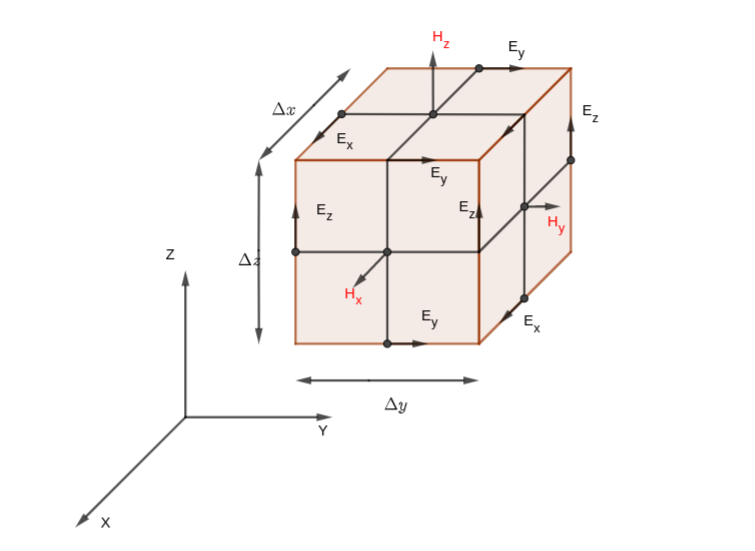
\includegraphics[width=0.7\linewidth]{figures/figure8}
	\caption{Field distribution on the basic space unit}
	\label{fig:figure8}
\end{figure}

In addition, it should be considered that E and H have a half time step change in time. Therefore, by introducing the differetial expression above, the scalar Maxwell's equations can also be rewritten into a differential form.

The solving steps of the FDTD numerical solution can be summarized as follows:

1. Expand Maxwell's curl equation in the time domain into its coordinate components. The central finite difference is used to replace the differentiation of each component field with respect to space and time, and the basic equation of FDTD is obtained.

2. Determine the basic unit size $\Delta x$, $\Delta y$ and $\Delta z$ of the spatial grid.

3. Choose the time step $\Delta t$. The choice of dt should ensure the stability of the numerical calculation, and its discriminant is

$$\Delta t \leq \frac{1}{c_{max}} \frac{1}{\sqrt{\frac{1}{\Delta x^2} + \frac{1}{\Delta y^2} + \frac{1}{\Delta z^2}}}$$

where $c_{max}$ is the maximum wave number of the mode that exists in the target space. In generally we choose $\Delta t = \Lambda / (2c_{max})$, $\Lambda$ is the minimum value among $\Delta x$, $\Delta y$ and $\Delta z$.

4. Determine the size of the target space and set the absorbing boundary conditions along the outer surface of the grid space. At the same time select and set the excitation source.

5. Determine the total number of time steps for the calculation and estimate the amount of storage for the calculation. When the storage capacity of the calculation is large, the calculation is generally performed on the server.

\section{Simulation subwavelength}
Simulation is one of the main contents of my internship research. By constructing the corresponding theoretical model on the computer, with the help of Lumerical and other software, we can easily obtain the characteristic parameters of the subwavelength structure or the grating structure. This not only provides me with high-precision theoretical results, but also saves my design time to a large extent. On this basis, I can also easily use sweep and other functions provided by the Lumerical to continuously optimize the simulation structure to obtain more suitable design parameters. In this part, I mainly simulated and optimized the three structures: L-shaped fiber-chip coupler, a symmetrical SOI waveguide with gradually changing width and Grating coupler with subwavelength structure arranged in matrix.

\subsection{L-shaped fiber grating coupler}
Firstly, I will study the L-shaped fiber-chip coupler, optimizing the related parameters and, at the same time, gradually mastering the use of Lumerical FDTD-solutions. It's worth mentioning, by adding a subwavelength structure at the beginning, the L-shaped fiber-chip coupler can provide a high coupler efficiency and a remarkably high grating directionality with a simplified fabrication process, compared with blazed gratings.



\begin{figure}[H]
	\centering
	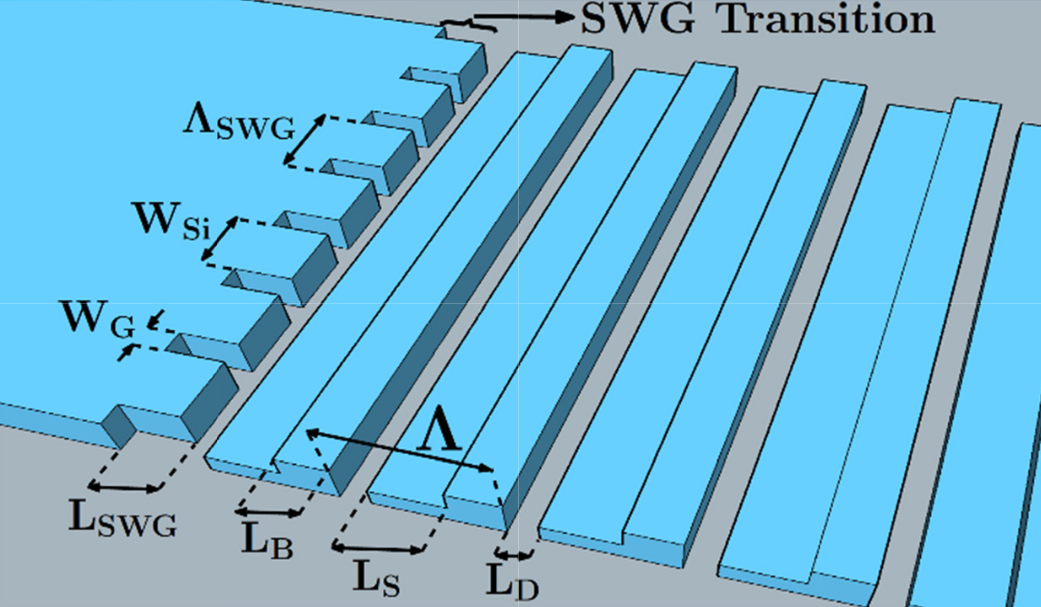
\includegraphics[width=0.7\linewidth]{figures/figure1}
	\caption{L-shaped fiber-chip coupler}
	\label{fig:figure1}
\end{figure}

The figure 1 above shows the 3D structure of the L-shaped fiber-chip coupler. The following simulation work based on this structure. The main purpose of my work for this structure is trying to reproduce the result mentioned in an article, to fulfill the high coupler efficiency and ultra direction. 

\subsubsection{Simulation setting}
For the convenience of description, I assume the direction in which the L-shape structure cycle repeats as x direction, the direction in which the subwavelength structure cycle repeats as z direction and the left as y directions. 

\begin{figure}[H]
	\centering
	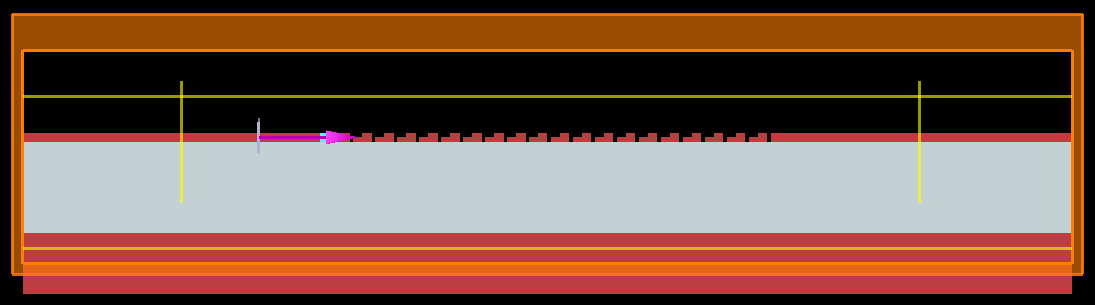
\includegraphics[width=0.7\linewidth]{figures/figure2}
	\caption{simulation model XY view}
	\label{fig:figure2}
\end{figure}

Refer to the parameter setting in figure 1, the grating coupler is implemented on a 300-nm-thick Si layer in 300 mm SOI wafer, relying on standard full (300 nm) and shallow (150 nm) etch steps. Here I set the length of the subwavelength part is $L_{SWG} = 255 nm$. The subwavelength period $\Lambda_{SWG} = 400 nm$ comprises the width of silicon $W_{si} = 300 nm$ and the width of gap $W_{gap} = 100nm$. The grating period $\Lambda = 720 nm$ comprises the deep- and shallow-etch trenches of lengths $L_D = 120 nm$ and $L_S = 290 nm$, respectively, and unetched Si block of length $L_B = 310nm$. The structure is optimized for transverse electrical (TE) mode, which means the polarization direction of the incident light is along the z direction. In the simulation, I create the FDTD for the whole input part, grating part and output part, setting the boundary condition as PML. Also I add 4 monitors. The monitor at the top of the grating is arranged to measure the energy of the diffracted light, which will be used to couple to a specific mode to calculate the coupler efficiency. And the monitors at the right and left are arranged to measure the transmitted energy and reflected energy.

\subsubsection{Result analysis}
Through the setting mentioned above, I can first directly get the energy received by the top monitor, left monitor and right monitor. One thing needs to pay attention that all the operation is in the C-band near 1.55 $\mu m$ (I take the wavelength from 1.5 $\mu m$ to 1.6 $\mu m$). 

\begin{figure}[H]
	\centering
	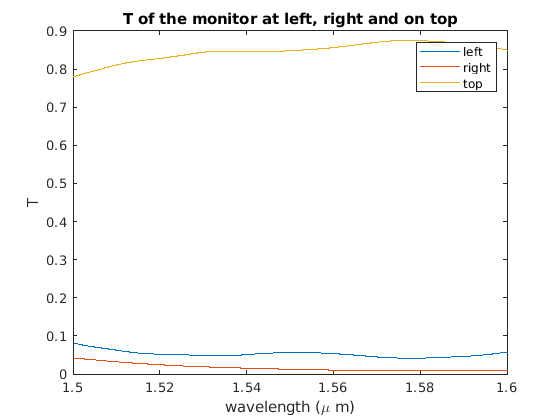
\includegraphics[width=0.7\linewidth]{figures/figure4}
	\caption{simulation model XY view}
	\label{fig:figure3}
\end{figure}

From the figure above we can see most of the energy is received by the monitor on the top. In fact it's a good sign, which means the grating coupler succeed in diffracting most of energy to a different plane (out of the waveguide transmission plane). This lays a solid foundation for excellent coupling efficiency in the future.

After knowing the information above, I tend to study the coupler proceed. Without affecting the generality, we can suppose to use this L-shaped grating coupler to couple the light on a chip to an optical fiber in the free space. Then the position (the angle of the fiber relative to the chip) and mode matching of the fiber will be critical to the coupling efficiency. This is because the proper position can ensure optical fiber to receive more energy of the diffracted light. The mode matching or not, on the other hand, determines whether the energy received can successfully enter the optical fiber for stable transmission. Here I consider the wavelength is 1.55 $\mu m$ and assume the light pulse transmitted in the optical fiber is a Gaussian pulse.

\begin{align*}
	Guassian_{norm,angle} = \frac{1}{\sqrt{I}}exp(\frac{-(x-x_0)^2}{\sigma^2})*exp(\frac{2i\pi n_{cladding}}{\lambda})*sin(\alpha)
\end{align*}

The $Gaussina_{norm,angle}$ present the normalized Gaussian pulse, where the $I$ is the optical intensity, $\lambda$ is the wavelength. From the formula above it's obvious to see that the position of the fiber will determine the value of $x_0$ and angle $\alpha$. On this basis, I can express the coupling efficiency as the product of Overlap and the amount of received light.

\begin{align*}
	Coupling \ efficiency = Overlap*T = |\int E_{z,norm} * (Gaussian_{norm,angle})^*dx|*T
\end{align*}

where the $E_{z,norm}$ is the electric filed of the light incident on the optical fiber, the T is the energy received by the top monitor (The T of the top monitor in figure 3).

Based on the above analysis, we can first consider the directionality of the L-shaped fiber-chip coupler. Through Lumerical FDTD-solutions, I can easily get the result of $Overlap$ with the change of angle and $x_0$.

\begin{figure}[H]
	\centering
	\subfigure[Overlap with $x_0$ and angle]{
	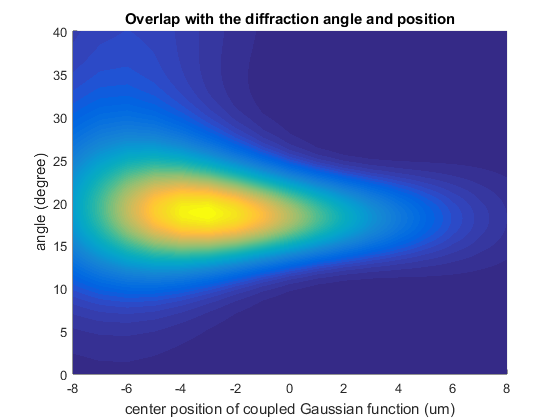
\includegraphics[width=0.48\linewidth]{figures/figure3}
	}
	\subfigure[Overlap with angle]{
	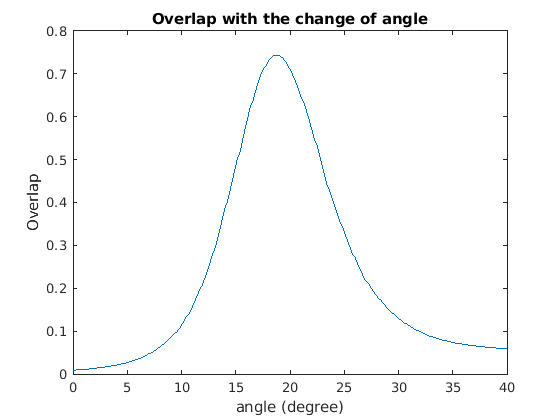
\includegraphics[width=0.48\linewidth]{figures/figure5}
	}
	\caption{Overlap}
	\label{fig:figure4}
\end{figure}

Here the figure present the change of Overlap with the change of angle and $x_0$. Also the figure 4-b directly present the relationship between angle and Overlap. It's worth mentioning when angle equals to $18.8^o$ the Overlap achieves its maximum value $0.7437$. This is ideal for my expectations. It provides the possibility for higher coupling efficiency. Then I take the best angle for overlap to calculate the coupling efficiency.

\begin{figure}[H]
	\centering
	\subfigure[Overlap with $x_0$ and angle]{
		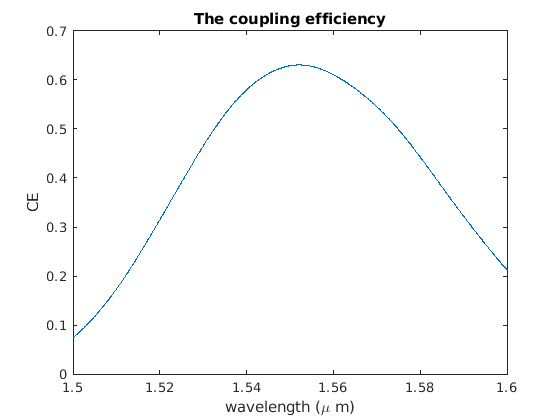
\includegraphics[width=0.48\linewidth]{figures/figure6}
	}
	\subfigure[Overlap with angle]{
		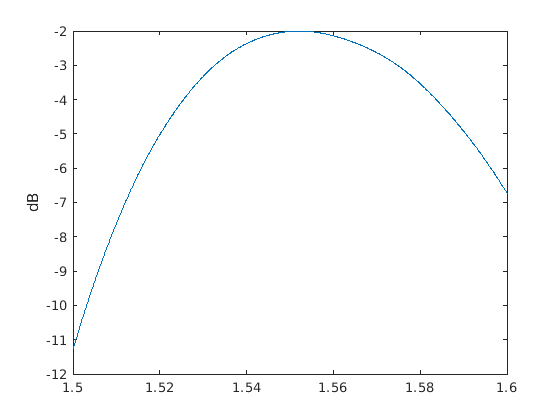
\includegraphics[width=0.48\linewidth]{figures/figure7}
	}
	\caption{Coupling efficiency}
	\label{fig:figure5}
\end{figure}

Here a simulation peak coupling efficiency is 0.6307 (-2.0015 dB) taken at 1552.1 nm. The -3 dB bandwidth is 42 nm.

\subsection{Grating coupler with subwavelength structure arranged in matrix}
In the end instead of adjusting the shallow etch depth of grating grooves to engineer the grating strength like what I've explained in the L-shaped fiber-chip coupler part, here using a fully etched SWG structure as was first proposed by Halir et al, which allows efficient grating apodization and simplifying fabrication.

\begin{figure}[H]
	\centering
	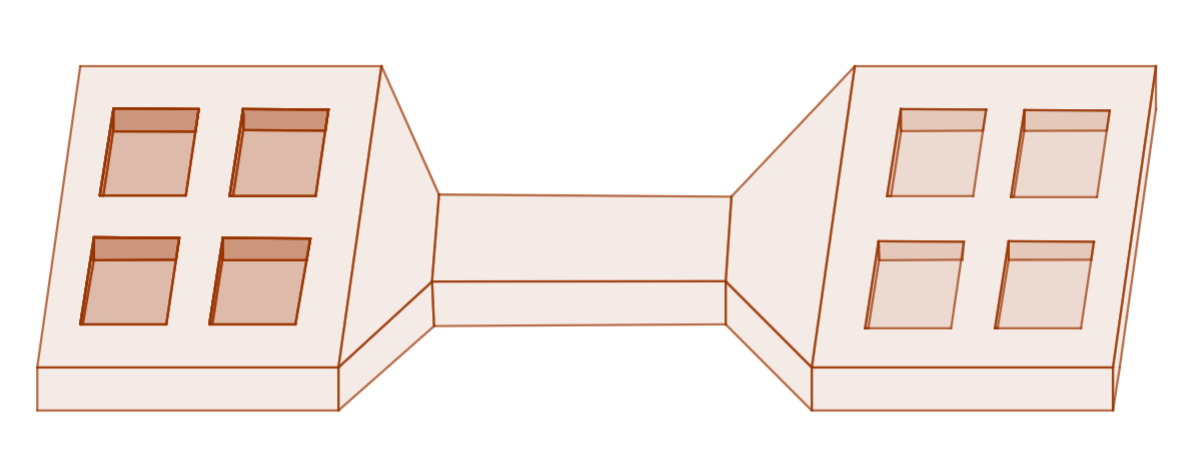
\includegraphics[width=0.7\linewidth]{figures/figure12.png}
	\caption{The grating structure}
	\label{fig:figure11}
\end{figure}

This structure should includes grating coupler part, a taper, a waveguide, a taper and a grating decoupler part. Below is the Decoupled two-dimensional models, illustrated in fig. a) and fig. b), are used in the yz-plane and xz-plane to model the diffractive grating and the SWG structure.

\begin{figure}[H]
	\centering
	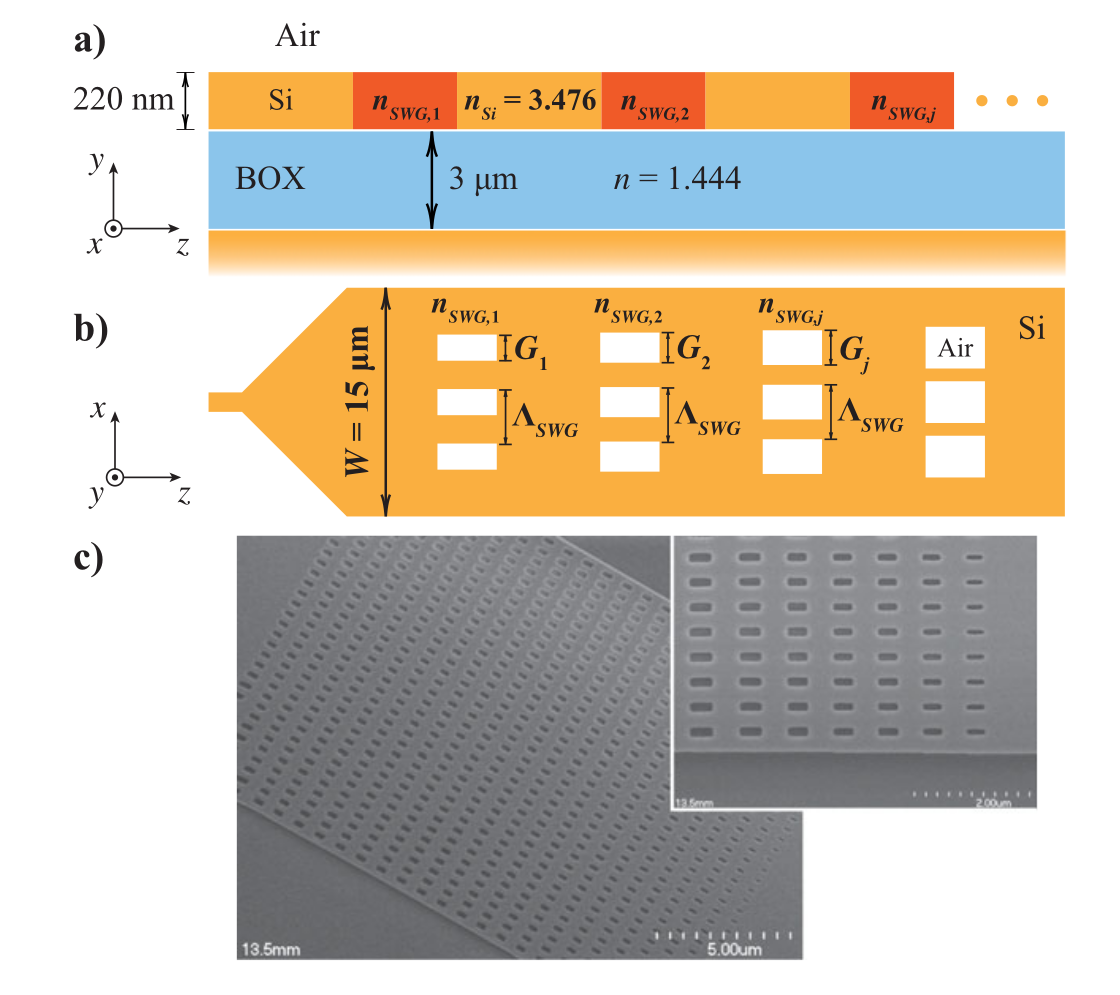
\includegraphics[width=0.7\linewidth]{figures/figure11.png}
	\caption{(a) Two-dimensional vertical cross-section schematic of SWG coupler. (b) Two-dimensional in-plane schematic of SWG coupler. (c) Scanning electron microscopy image of fabricated continuously apodized coupler. Inset: detailed view.}
	\label{fig:figure11}
\end{figure}

The SWG is a periodic structure implemented by interleaving two constituent materials, here silicon and air, with refractive indices $n_{Si} = 3.476$ and $n_{air} = 1$. Here I assume the light transmits in z direction and then coupled to a optical fiber above the coupler by the grating structure. The width of the SWG structure should be $W = 15 \mu m$ and the length of the whole grating part should be $L = 40 \mu m$. Then I note the width (in x direction) of the air gap and silicon gap as $W_{air}$ and $W_{Si}$, the length (in z direction) of the air gap and silicon gap as $L_{air}$ and $L_{Si}$. 

\subsubsection{Building simulation structure}

According to the previous analysis, it can be known that this kind of long periodic structure (which can form multiple resonant cavities) is almost impossible to run 3 dimensional simulation in Lumerical. Therefore, it is very important to simplify the target structure to achieve two-dimensional simulation, which means the structure should be changed to be invariant in the x direction. Therefore, in the z direction, for the periodic part of the structure that contains air, we can equate it to a substance with a refractive index of $n_{SWG}$ (as in figure11 (a)). Obviously, the value of $n_{SWG}$ should be between $n_{air}$ and $n_{Si}$, and is determined by the duty cycle in the x direction. From this perspective, in the simulation, $n_{SWG}$ can be assigned directly, and when optimized to the optimal situation (to get the best coupling efficiency), the values of $n_{air}$ and $n_{Si}$ are determined according to the corresponding $n_{SWG}$ value. This not only simplifies the simulation process but also greatly saves simulation time. Below is the model I used in the Lumerical FDTD-solutions.

\begin{figure}[H]
	\centering
	\subfigure[yz-plane]{
		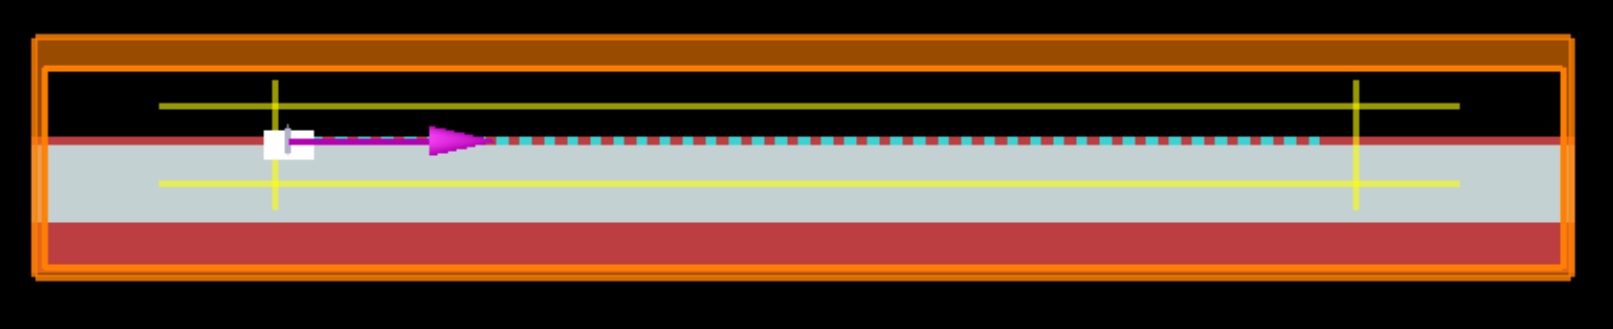
\includegraphics[width=0.8\linewidth]{figures/figure13}
	}
	\subfigure[xz-plane]{
		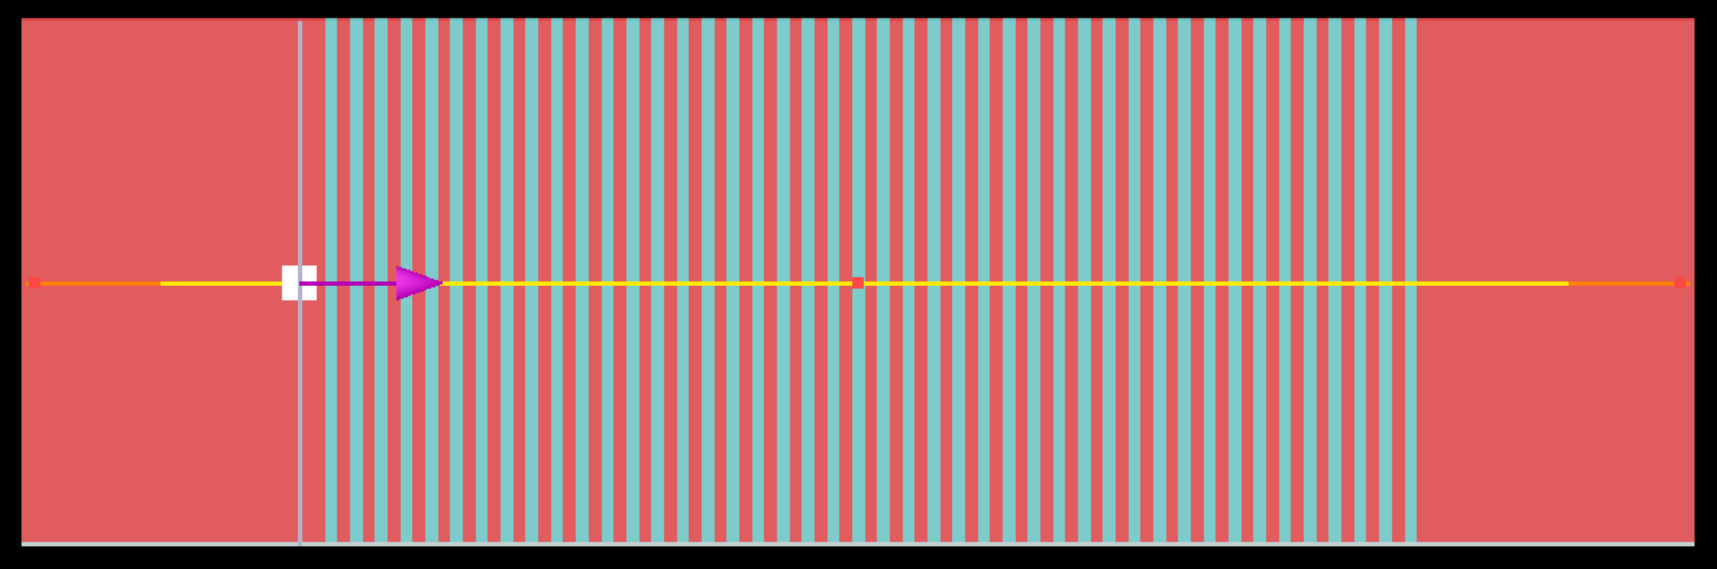
\includegraphics[width=0.8\linewidth]{figures/figure14}
	}
	\caption{The simulation model of the decoupler grating part}
	\label{fig:figure5}
\end{figure}

The following is optimized for the above structure, mainly adjusting $n_{SWG}$, $L_{Si}$ and $L_{air}$, hoping to obtain the best coupling efficiency. The target wavelength is 1.55 $\mu m$.

\subsubsection{Normalized structural parameters}

Here I firstly consider normalized structural parameters,the simplest situation, which means that I keep all $n_{SWG}$ the same value in the z direction. Considering the $n_{SWG}$ should be bigger than the $n_{air}$ and smaller than the $n_{Si}$, I take $n_{SWG} = 2.2, 2.3, 2.4,..., 2.8$. Then for the length of the silicon and air, I keep them change in the range of 0.21 $\mu m$ to 0.45 $\mu m$, with the step equal to $0.03 \mu m$. After that, I calculated every combination of $n_{SWG}$, $L_{si}$, and $L_{gap}$ in Lumerical, and checked the light energy received by each monitor (top, left, right). 

% a figure here

\begin{figure}[H]
	\centering
	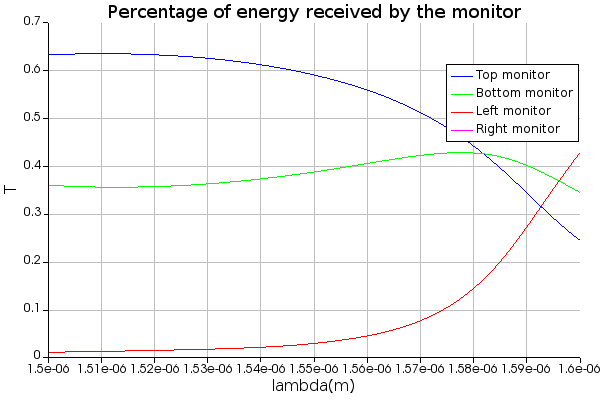
\includegraphics[width=0.7\linewidth]{figures/figure15.png}
	\caption{ $n_{SWG} = 2.4$, $L_{si} = 0.3 \mu m$ and $L_{air} = 0.36 \mu m$}
	\label{fig:figure11}
\end{figure}

Similar to the content shown in 4.1, suppose an optical fiber is located above grating, assuming the transmission mode in the optical fiber to Gaussian distribution, then calculate the overlap and coupling efficiency. Here I note the value of $n_{SWG}$, $L_{Si}$ and $L_{air}$ for the maximum overlap and maximum coupling efficiency. Also noting the coupling angle for the two situations.

\begin{table}[htbp]
	\centering
	\caption{Best  combination of $n_{SWG}$, $L_{Si}$ and $L_{air}$ for normalized structure}
	\begin{tabular}{cccccc}
		\hline
		target & target value & angle (degree) & $n_{SWG}$ & $L_{si} (\mu m)$ & $L_{air} (\mu m)$ \\ \hline
		maximize CE & 0.4796 & 7.5 & 2.4 & 0.30 & 0.36 \\
		maximize OL & 0.8256 & 0.9 & 2.4 & 0.27 & 0.36 \\ \hline
	\end{tabular}
\end{table}

Below is the corresponding result of Overlap and Coupling efficiency.

\begin{figure}[H]
	\centering
	\subfigure[Overlap of the best combination of $n_{SWG}$, $L_{Si}$ and $L_{air}$ maximizing CE]{
		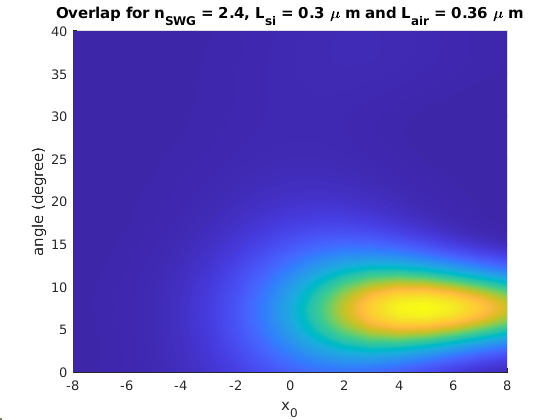
\includegraphics[width=0.48\linewidth]{figures/figure16}
	}
	\subfigure[The coupling efficiency of best $x_0$ and $angle$ to maximize Overlap at left]{
		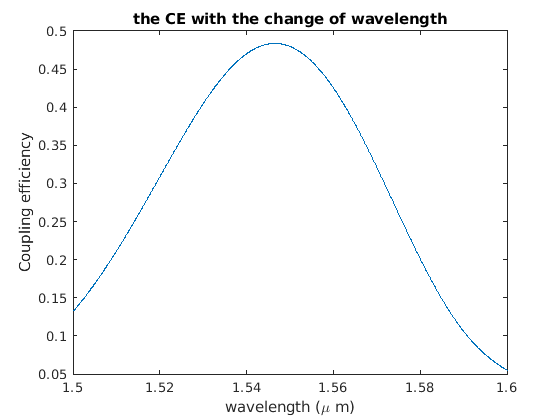
\includegraphics[width=0.48\linewidth]{figures/figure17}
	}
	\caption{The simulation model of the decoupler grating part}
	\label{fig:figure5}
\end{figure}





\subsubsection{Apodization optimization}

Above I've achieved an around -3 dB coupling efficiency. However, there is still a lot of room for optimization. In mathematics, the rearrangement inequality tells how to find the maximum value for a product sum. For every choice of real numbers

$$x_1 \leq x2 \leq ... \leq x_n \text{ and } y_1 \leq y2 \leq ... \leq y_n \, ,$$

and every permutation

$$x_{\sigma (1)}, x_{\sigma (2)},...,x_{\sigma (n)} \text{ of } x_1, x_2, ..., x_n \, ,$$

the rearrangement inequality states that 

$$x_ny_1 + x_{n-1}y_2 + ... + x_1y_n \leq x_{\sigma (1)}y_1 + x_{\sigma (2)}y_2 + ... + x_{\sigma (n)}y_n \leq x_1y_1 + x_2y_2 + ... + x_ny_n \, .$$

Then we review the formula for calculating coupling efficiency

\begin{align*}
	Coupling \ efficiency = Overlap*T = |\int E_{z,norm} * (Gaussian_{norm,angle})^*dx|*T
\end{align*}


Through comparison, it can be found that in order to make the value of coupling efficiency as large as possible, it is necessary to ensure that the distribution of $E_z$ and $Gaussian function$ satisfies the nature of the rearrangement inequality. In other words, the distribution of the $E_z$ is expected to be similar to Gaussian distribution. However, the previous normalization parameters make the overall structure appear consistent. Therefore, for the monitor located on grating, the received light intensity gradually decreases in the propagation direction. That is, $E_z$ decreases monotonously. This obviously does not correspond to the previous analysis. Therefore, you can consider changing the structural parameters of the first few cycles of grating to make it less "perfect". So that $E_z$ has a gradual increase in the propagation direction first, and then gradually decreases. Therefore, the distribution of $E_z$ is similar to the Gaussian distribution, and theoretically, a better coupling efficiency can be obtained.

% 基于以上想法,我将grating沿光传播方向分为两个部分。前一部分包含NA个周期,后一部分则为grating的剩余的部分。此时保持后半部分的参数与之前的最优归一化参数相同。而对于前NA个周期,当NA取不同值时,再次寻找合适的nSWG, Lsi 和 Lair 的组合,找出最大耦合效率与其对应的组合。
Based on the above ideas, I divided grating into two parts along the light propagation direction. The former part contains NA cycles, and the latter part is the remaining part of the grating. At this time, keep the parameters ($n_{SWG}$, $L_{si}$ and $L_{air}$) of the latter part the same as the previous optimal normalized parameters. For the previous NA cycles, when NA takes a different value, look for different combination of $n_{SWG}$, $L_{si}$ and $L_{air}$ again to find the maximum coupling efficiency and its corresponding combination. Here I take $NA = 2, 3, 4, 5, 6, 7 to do the simulation$. The range of $n_SWG$, $L_{Si}$ and $L_{air}$ is also the same as before.    

\hspace*{\fill} 

\begin{table}[htbp]
	\centering
	\caption{Apodization optimization}
	\begin{tabular}{cccccc}
		\hline
		NA & target & target value & $n_{SWG}$ & $L_{si}(\mu m)$ & $L_{air}(\mu m)$ \\ \hline
		2 & max CE & 0.5141 & 2.7 & 0.27 & 0.36 \\
		3 & max CE & 0.5201 & 2.7 & 0.3 & 0.33 \\
		4 & max CE & 0.5253 & 2.7 & 0.3 & 0.33 \\
		5 & max CE & 0.5309 & 2.8 & 0.3 & 0.33 \\
		6 & max CE & 0.5287 & 2.8 & 0.3 & 0.3 \\
		7 & max CE & 0.5310 & 2.8 & 0.3 & 0.3 \\ \hline
	\end{tabular}
\end{table}

\hspace*{\fill} 

From the above results, it can be seen that the coupling efficiency after optimization has improved slightly, but it is difficult to find a trend from it. At this time, there are only three cases for the corresponding combination of $n_SWG$, $L_{Si}$ and $L_{air}$, corresponding to NA = 2, NA = 3, 4, 5, NA = 6, 7. The following uses the values of $n_SWG$, $L_{Si}$ and $L_{air}$ corresponding to these three sets of data to record the changes in coupling efficiency by changing the value of NA.

\begin{figure}[H]
	\centering
	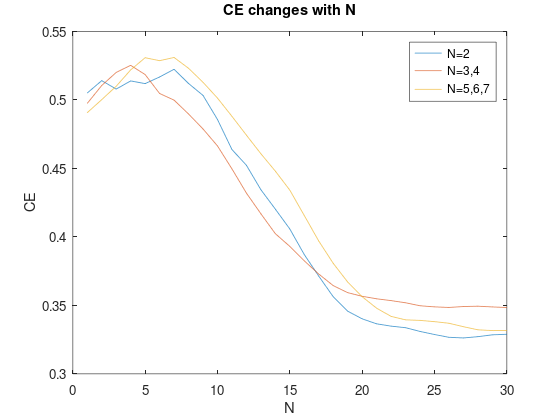
\includegraphics[width=0.7\linewidth]{figures/figure20.png}
	\caption{ $n_{SWG} = 2.4$, $L_{si} = 0.3 \mu m$ and $L_{air} = 0.36 \mu m$}
	\label{fig:figure11}
\end{figure}

Observing the above results, it can be found that the coupling efficiency has been improved after the preliminary optimization, but the improvement is not very ideal. The maximum value of coupling efficiency, which is often obtained between NA = 4 and NA = 8, is always smaller than 0.54.


\subsubsection{Continuous Apodization optimization}

In fact, this result above is predictable. Because the optimization of the structure is too simple, it is only the splicing of two different normalized structures. It is conceivable that the function characteristic of the light intensity received by the monitor in the light propagation direction should be the splicing of two monotonically decreasing functions. In this case, the received light intensity distribution obviously cannot present the characteristics of Gaussian distribution perfectly. Therefore, in order to further improve the coupling efficiency, more detailed optimization of the structure is required. By changing the structural parameters of each period in the previous NA periods, continuous apodization of the grating can be realized. In this way, the light intensity received by the detector can gradually increase in the propagation direction (corresponding to first NA periods), then combined with the monotonically decreasing distribution of the second part, I can finally make the light intensity distribution present the very similar shape of Gaussian distribution. 


\section{Create structures in Graphic Data System (GDS)}


\subsection{GDS introduction}

\subsection{GDSPY in Python}

\section{Measurement}

\newpage

\begin{thebibliography}{99}
\bibitem{ref1}asdad
\end{thebibliography}


\end{document}

